\section{Particles and Fluids}
We have directly ported our previous particle project in this fluid project. The velocity field can exert forces onto the particles. This is done by introducing two new forces, pressure and drag.\\
The pressure force is initialised for each particle. At the update step the position of the particle is determined. The density and velocity on this position are calculated using the same formula as the advection step in the fluid simulator. The added force on the particle is $ f_{pres} = (velocity*factor) * density * damp$, where $factor$ and $damp$ are constants. The density is included so the particle will only be moved when a is fluid present.\\
The drag force is used to slow the particle down when there is no fluid present anymore. At each update step the following force is added: $f_{drag} = drag * -velocity$, where $drag$ is a constant and $velocity$ the current velocity of the particle. In figure \ref{fig:cloth} it can be seen how the fluid influences two pieces of cloth.

\begin{figure}[!htb]
    \centering
    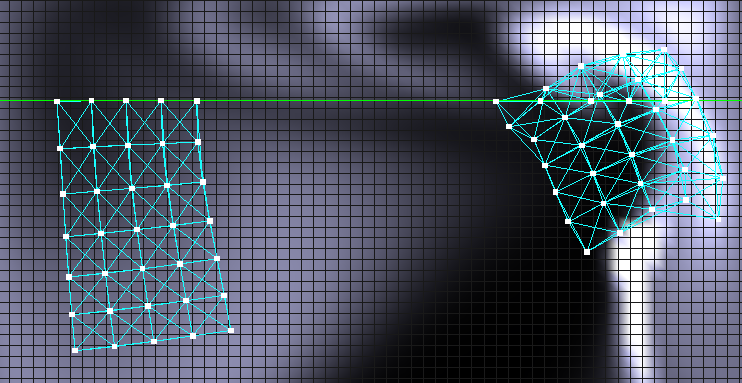
\includegraphics[width=10cm]{img/cloth.png}
    \caption{A piece of cloth interaction with the fluid.}
    \label{fig:cloth}
\end{figure}
